% ============================================================
%  SITEE 2026 — IEEE conference format, 3–4 pages
% ============================================================
\documentclass[conference]{IEEEtran}
\IEEEoverridecommandlockouts

\usepackage[T1]{fontenc}
\usepackage[utf8]{inputenc}
\usepackage{amsmath,amssymb}
\usepackage{booktabs}
\usepackage{xcolor}
\usepackage{pgfplots}
\usepackage{tikz}
\usepackage{microtype}
\usepackage{cite}
\usepackage{url}
\usepackage{subfig}
\usepackage{array}
\usepackage{enumitem}

\pgfplotsset{compat=1.18}
\usetikzlibrary{positioning, arrows.meta, calc}

% ── Palette ──────────────────────────────────────────────────
\definecolor{clrBlue}   {HTML}{1565C0}
\definecolor{clrOrange} {HTML}{E65100}
\definecolor{clrGreen}  {HTML}{2E7D32}
\definecolor{clrBoxA}   {HTML}{DCEEFB}
\definecolor{clrBoxB}   {HTML}{D7EDDA}

% ── Layout ───────────────────────────────────────────────────
\renewcommand{\arraystretch}{1.08}
\setlist[itemize]{nosep,leftmargin=1.2em}
\setlist[enumerate]{nosep,leftmargin=1.5em}

% ── Variant label commands ───────────────────────────────────
\newcommand{\Vpacked}{\textsf{Packed}}
\newcommand{\Vbase}{\textsf{Baseline}}
\newcommand{\Voz}{\textsf{OpenZeppelin}}
\newcommand{\Vopt}{\textsf{Optimized}}

% =============================================================
\begin{document}

\title{On-Chain Diploma Verification on Ethereum:\\
Cost Trade-Offs Between Per-Record Storage\\
and Merkle-Batch Architectures}

\author{
  \IEEEauthorblockN{Nazar Shcherbyna}
  \IEEEauthorblockA{
    Faculty of Electrical Engineering\\
    Warsaw University of Technology, Warsaw, Poland\\
    \texttt{nazar.shcherbyna.stud@pw.edu.pl}
  }
}

\maketitle

% =============================================================
\begin{abstract}
This paper presents UniVerify, a prototype system for
issuing, verifying, and revoking academic diplomas on
Ethereum. The study compares two on-chain representations:
\emph{a packed per-record benchmark baseline}, where each
diploma occupies one packed storage slot, and
\emph{Merkle batch issuance}, where an entire graduation
cohort is represented by a single Merkle root.

To separate architectural and implementation effects, four
contract variants are benchmarked:
a packed per-record model (\Vpacked{}),
a custom Solidity Merkle implementation (\Vbase{}),
the OpenZeppelin MerkleProof library (\Voz{}),
and an assembly-optimized Merkle variant (\Vopt{}).
Measurements cover proof depths
$d \in \{0,1,4,8,10,12\}$.

Merkle batching reduces per-diploma issuance cost by
98.9\% at batch size $N=100$, while shifting part of the
cost to proof-based verification.
Compared with \Vbase{}, \Vopt{} lowers verification gas by
6.6\%, and by 3.7\% relative to \Voz{}.
A closed-form gas-savings model is derived and validated at
six proof depths, with residuals below 0.2\%.
Under an illustrative mainnet scenario
(40~gwei, 1\,ETH\,=\,\$2{,}500), issuing 1{,}000 diplomas
costs about \$4{,}820 with per-record storage versus about
\$5.1 with Merkle batching.
Overall, the results indicate that for institutional
diploma issuance, batching has a much larger impact on
practical cost than low-level micro-optimization.
\end{abstract}

\begin{IEEEkeywords}
Ethereum, Solidity, gas optimization, Merkle tree,
smart contracts, diploma verification
\end{IEEEkeywords}

% =============================================================
\section{Introduction}
\label{sec:intro}

Academic credential verification remains largely
institution-centric.
Cross-border or post-graduation checks often require manual
contact with the issuing university, which makes the
process slow and difficult to automate.
At the same time, forged diplomas remain a persistent
problem~\cite{ezell2012degree}.
Blockchain-based registries offer an alternative:
once a credential commitment is published on-chain, any
verifier can validate authenticity independently, without
relying on a single institutional database.

The main challenge is economic.
On Ethereum, persistent storage writes are expensive.
If each diploma is stored individually, the university pays
for one state update per record.
For institutions issuing hundreds or thousands of diplomas
per cycle, this quickly becomes the dominant cost.
The key question is therefore not whether blockchain can be
used, but \emph{how credentials should be represented
on-chain so that issuance remains practical}.

This paper studies that question in the context of
\emph{UniVerify}, a prototype diploma-verification system.
Two architectures are compared:
\begin{enumerate}
  \item \textbf{Per-record storage}, where each diploma is
        stored in its own mapping slot and verified in
        constant time.
  \item \textbf{Merkle batch issuance}, where one Merkle
        root represents an entire batch and each diploma is
        verified using an off-chain proof.
\end{enumerate}

The contribution is practical rather than conceptual.
Rather than proposing a new credential format, this work
quantifies the gas implications of deployable Solidity
designs and asks:
\emph{when does batching make on-chain diploma registries
economically viable?}

\subsection{UniVerify System}

UniVerify is a prototype system for issuing, verifying,
and revoking academic diplomas on Ethereum.
It consists of:
\begin{itemize}
  \item a \textbf{Solidity smart contract} for on-chain
        storage, verification, and revocation;
  \item an \textbf{off-chain TypeScript SDK} for hashing,
        Merkle tree construction, and proof generation;
  \item a \textbf{web application} for issuers, verifiers,
        and administrators;
  \item a \textbf{REST API} for integration with university
        information systems.
\end{itemize}

Universities act as \emph{issuers} who publish diploma
commitments on-chain.
A verifier later checks a diploma using the document hash
and, in the Merkle variant, a proof of inclusion in the
published batch root. In the current UniVerify contract,
the final \texttt{Valid} decision also depends on whether
the issuer remains linked to an active university at the
time of verification.

\subsection{Contributions}

\begin{enumerate}
  \item A quantitative comparison between a packed
        per-record benchmark baseline and a Merkle-batch
        UniVerify registry across issuance, verification,
        revocation, and deployment cost.
  \item A four-way benchmark of \Vpacked{}, \Vbase{},
        \Voz{}~\cite{openzeppelin}, and \Vopt{}, separating
        architectural, library-level, and low-level EVM
        effects.
  \item A closed-form gas-savings model for the optimized
        Merkle path, validated experimentally at six proof
        depths with residuals below 0.2\%.
  \item An economic interpretation showing how gas savings
        translate into institutional issuance cost.
\end{enumerate}

% =============================================================
\section{Related Work}
\label{sec:related}

Grech and Camilleri~\cite{grech2017blockchain} identified
credential verification as one of the main educational
applications of blockchain.
Lizcano et~al.~\cite{lizcano2020decentralised} proposed a
decentralized framework for academic credentials based on
IPFS and Ethereum, but without low-level cost analysis.
Alketbi et~\cite{alketbi2018blockchain} discussed broader
blockchain use in public-sector services, including
education records.

Merkle trees~\cite{merkle1987} are the standard mechanism
for compact set-membership proofs.
OpenZeppelin's \texttt{MerkleProof}~\cite{openzeppelin}
serves as the de facto production Solidity library.
Alternative authenticated data structures, including sparse
Merkle trees, Verkle trees~\cite{verkle}, and RSA
accumulators, remain interesting but less practical for
ordinary EVM contracts.

Ethereum execution costs are determined by the EVM gas
schedule~\cite{yellowpaper}.
In particular, EIP-2929 increased the cost of cold state
accesses, directly affecting storage-based lookups
\cite{eip2929}.
Most prior work on blockchain credentials emphasizes
system architecture, privacy, governance, or
interoperability.
By contrast, this paper studies a narrower but practically
important question: how specific Solidity design choices
change issuance and verification cost in a deployable
credential-registry prototype.

% =============================================================
\section{System Design and Methodology}
\label{sec:method}

\subsection{Two Verification Architectures}

The two approaches are illustrated in
Fig.~\ref{fig:arch}.

\smallskip\noindent\textbf{Architecture A --- Per-Record Storage.}
For benchmarking, each diploma is stored in a
\texttt{mapping(bytes32\,$\Rightarrow$\,uint256)}.
The issuer address (160~bits) and a revocation flag (1~bit)
are packed into one 256-bit slot.
Issuance requires one \texttt{SSTORE} per diploma.
Verification is a single \texttt{SLOAD} plus bit masking,
so read cost is constant. This contract is intentionally
minimal and serves as a gas baseline rather than a
feature-equivalent version of the full UniVerify registry.

\smallskip\noindent\textbf{Architecture B --- Merkle Batch.}
All diplomas in a cohort are arranged into a Merkle tree
off-chain.
Only the 32-byte batch root is stored on-chain via
\texttt{issueBatchRoot}, so one state write covers the
entire batch.
Verification requires the caller to provide
$d=\lceil \log_2 N \rceil$ sibling hashes, shifting cost
from storage to proof processing.
Each leaf is domain-separated:
$\texttt{keccak256}(\mathit{contract}\|\mathit{chainId}
\|\mathit{issuer}\|\mathit{batchId}\|\mathit{docHash})$,
which prevents cross-contract and cross-chain replay.

% ── FIGURE: Architecture comparison ─────────────────────────
\begin{figure}[t]
\centering
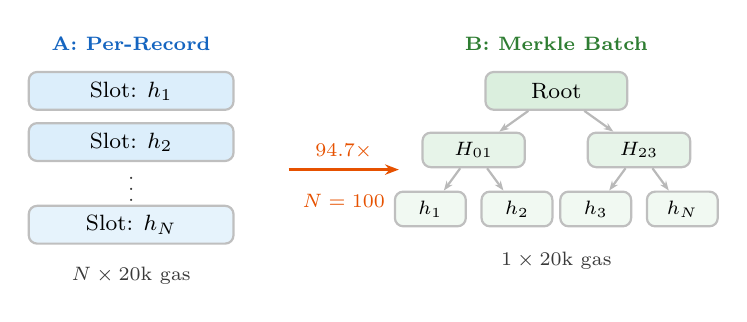
\begin{tikzpicture}[
  box/.style={draw=gray!50, rounded corners=3pt,
              minimum width=2.6cm, minimum height=0.48cm,
              font=\footnotesize, align=center, thick},
  arr/.style={-{Stealth[length=3.5pt]}, thick, gray!55},
  lbl/.style={font=\scriptsize\bfseries},
  note/.style={font=\scriptsize, text=gray!45!black},
]
\node[lbl, text=clrBlue] at (-2.7, 2.6) {A: Per-Record};
\node[box, fill=clrBoxA] (a1) at (-2.7, 2.0) {Slot: $h_1$};
\node[box, fill=clrBoxA] (a2) at (-2.7, 1.35) {Slot: $h_2$};
\node[note] at (-2.7, 0.85) {$\vdots$};
\node[box, fill=clrBoxA!70] (aN) at (-2.7, 0.3) {Slot: $h_N$};
\node[note, align=center] at (-2.7, -0.35)
  {$N \times 20\text{k gas}$};

\node[lbl, text=clrGreen] at (2.7, 2.6) {B: Merkle Batch};
\node[box, fill=clrBoxB!90, minimum width=1.8cm] (root)
  at (2.7, 2.0) {Root};
\node[box, fill=clrBoxB!60, minimum width=1.3cm,
      minimum height=0.38cm, font=\scriptsize]
  (h1) at (1.65, 1.25) {$H_{01}$};
\node[box, fill=clrBoxB!60, minimum width=1.3cm,
      minimum height=0.38cm, font=\scriptsize]
  (h2) at (3.75, 1.25) {$H_{23}$};
\node[box, fill=clrBoxB!35, minimum width=0.9cm,
      minimum height=0.32cm, font=\scriptsize]
  (l0) at (1.1, 0.5) {$h_1$};
\node[box, fill=clrBoxB!35, minimum width=0.9cm,
      minimum height=0.32cm, font=\scriptsize]
  (l1) at (2.2, 0.5) {$h_2$};
\node[box, fill=clrBoxB!35, minimum width=0.9cm,
      minimum height=0.32cm, font=\scriptsize]
  (l2) at (3.2, 0.5) {$h_3$};
\node[box, fill=clrBoxB!35, minimum width=0.9cm,
      minimum height=0.32cm, font=\scriptsize]
  (l3) at (4.3, 0.5) {$h_N$};
\draw[arr] (root)--(h1); \draw[arr] (root)--(h2);
\draw[arr] (h1)--(l0);   \draw[arr] (h1)--(l1);
\draw[arr] (h2)--(l2);   \draw[arr] (h2)--(l3);
\node[note, align=center] at (2.7, -0.15)
  {$1 \times 20\text{k gas}$};

\draw[very thick, clrOrange, -{Stealth[length=5pt]}]
  (-0.7, 1.0) -- node[above, font=\scriptsize\bfseries,
  text=clrOrange] {$94.7\times$} (0.7, 1.0);
\node[note, text=clrOrange] at (0.0, 0.6) {$N=100$};
\end{tikzpicture}
\caption{Comparison of on-chain issuance models.
Per-record storage writes one slot per diploma, whereas
Merkle batching writes one root for the whole cohort.}
\label{fig:arch}
\end{figure}

\subsection{Contract Variants}
\label{sec:variants}

To distinguish architectural effects from implementation
effects, four contract variants were implemented
(Table~\ref{tab:variants}).

\begin{table}[t]
\centering
\caption{Contract Variants}
\label{tab:variants}
\setlength{\tabcolsep}{3.5pt}
\begin{tabular}{@{}llp{3.6cm}@{}}
\toprule
Label & Architecture & Key implementation detail \\
\midrule
\Vpacked{}
  & Per-record
  & Packed \texttt{uint256} slot: issuer address (160\,b)
    + revocation flag (1\,b) \\[3pt]
\Vbase{}
  & Merkle batch
  & Hand-written proof traversal and leaf construction
    using \texttt{abi.encodePacked} \\[3pt]
\Voz{}
  & Merkle batch
  & Uses OpenZeppelin
    \texttt{MerkleProof.verifyCalldata} \\[3pt]
\Vopt{}
  & Merkle batch
  & Four EVM-level optimizations (T1--T4) applied
    to the verification hot path \\
\bottomrule
\end{tabular}
\end{table}

\subsection{Optimization Techniques}
\label{sec:techniques}

The \Vopt{} variant targets two internal functions used
during proof verification:
\texttt{\_processProof()} and \texttt{\_merkleLeaf()}.

\smallskip\noindent\textbf{T1 --- Unchecked loop arithmetic.}
Wrapping the loop increment in
\texttt{unchecked\{++i;\}} removes overflow-check overhead.

\smallskip\noindent\textbf{T2 --- Scratch-space keccak256.}
Instead of \texttt{abi.encodePacked(a,b)}, the two 32-byte
inputs are written directly to EVM scratch space and hashed
in place, avoiding repeated memory allocation.

\smallskip\noindent\textbf{T3 --- Validation path splitting.}
The public \texttt{merkleLeaf()} performs input checks,
while a private \texttt{\_merkleLeaf()} is used internally.

\smallskip\noindent\textbf{T4 --- Assembly preimage packing.}
The 112-byte leaf preimage is packed manually with
\texttt{mstore}/\texttt{shl} instead of
\texttt{abi.encodePacked}.

\subsection{Experimental Setup}

All measurements were collected with
Foundry~\cite{foundry2023} using Solidity~0.8.20 with the
optimizer enabled at 200 runs.
Merkle trees were constructed on-chain only inside the test
harness; in deployment they are built off-chain.
Proof depths $d \in \{0,1,4,8,10,12\}$ correspond to batch
sizes from $2^0$ to $2^{12}$ (1 to 4{,}096 diplomas).
Gas was measured with
\texttt{forge test --gas-report}; the reported values are
function-level gas figures from Foundry's gas report rather
than full end-to-end test-harness cost.

% ── FIGURE*: dual panel ───────────────────────────────────────
\begin{figure*}[t]
\centering
\subfloat[Per-diploma issuance cost.
  \Vpacked{} is constant at 48{,}200~gas, while the
  Merkle cost decays as $50{,}939/N$.]{%
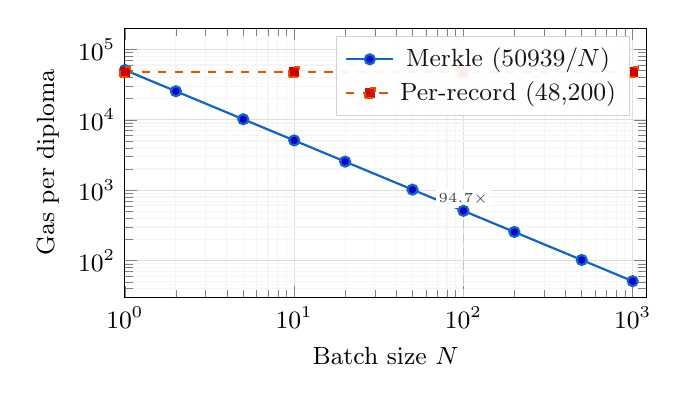
\begin{tikzpicture}
\begin{axis}[
  width=8.2cm, height=5cm,
  xlabel={Batch size $N$},
  ylabel={Gas per diploma},
  xmode=log, ymode=log,
  log basis x=10, log basis y=10,
  xmin=1, xmax=1200, ymin=30, ymax=200000,
  grid=both,
  minor grid style={gray!8},
  major grid style={gray!25},
  legend style={at={(0.97,0.97)}, anchor=north east, font=\small,
    fill=white, fill opacity=0.92, draw=gray!35},
  tick label style={font=\small},
  label style={font=\small},
]
\addplot+[mark=*, thick, color=clrBlue, mark size=1.8pt]
  coordinates {(1,50939)(2,25470)(5,10188)(10,5094)(20,2547)
               (50,1019)(100,509)(200,255)(500,102)(1000,51)};
\addlegendentry{Merkle ($50939/N$)}
\addplot+[mark=square*, thick, color=clrOrange, dashed,
          mark size=1.8pt]
  coordinates {(1,48200)(10,48200)(100,48200)(1000,48200)};
\addlegendentry{Per-record (48{,}200)}
\draw[densely dashed, gray!45]
  (axis cs:100,30)--(axis cs:100,509);
\node[font=\tiny, text=gray!55!black, fill=white, inner sep=1pt]
  at (axis cs:100,750) {$94.7\times$};
\end{axis}
\end{tikzpicture}%
\label{fig:amort}%
}
\hfill
\subfloat[Closed-form model~\eqref{eq:model} versus
  measured gas savings (\Vbase{}\,$-$\,\Vopt{}).]{%
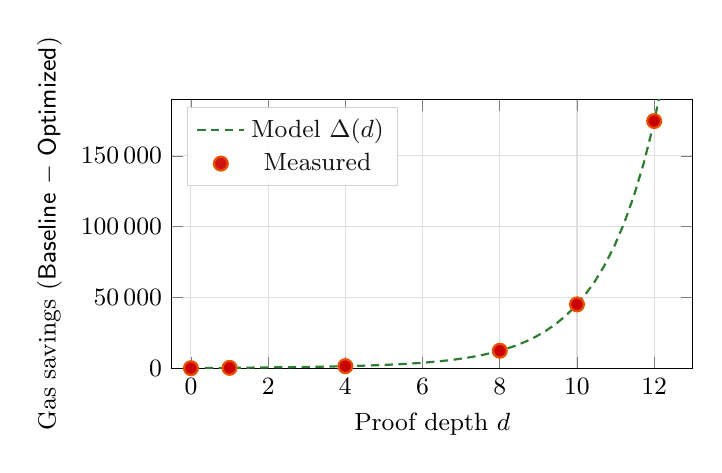
\begin{tikzpicture}
\begin{axis}[
  width=8.2cm, height=5cm,
  xlabel={Proof depth $d$},
  ylabel={Gas savings (\Vbase{} $-$ \Vopt{})},
  xmin=-0.5, xmax=13, ymin=0, ymax=190000,
  grid=both,
  minor grid style={gray!8},
  major grid style={gray!25},
  legend style={at={(0.03,0.97)}, anchor=north west, font=\small,
    fill=white, fill opacity=0.92, draw=gray!35},
  tick label style={font=\small},
  label style={font=\small},
  scaled y ticks=false,
  yticklabel style={/pgf/number format/fixed,
                    /pgf/number format/1000 sep={\,}},
]
\addplot+[thick, densely dashed, color=clrGreen, mark=none,
  domain=0:12.5, samples=50] {2^x * 42 + 96 + x*199 + 42};
\addlegendentry{Model $\Delta(d)$}
\addplot+[only marks, mark=*, mark size=2.5pt, thick,
          color=clrOrange]
  coordinates {(0,180)(1,421)(4,1606)(8,12484)
               (10,45218)(12,174641)};
\addlegendentry{Measured}
\end{axis}
\end{tikzpicture}%
\label{fig:model}%
}
\caption{Main results:
(a) issuance-cost amortization and
(b) validation of the closed-form savings model.}
\label{fig:results}
\end{figure*}

% =============================================================
\section{Results}
\label{sec:results}

\subsection{Issuance Cost}

Table~\ref{tab:amort} compares per-diploma issuance cost.
In the Merkle architecture, publishing one batch root costs
50{,}939~gas regardless of batch size, so the amortized
cost is $50{,}939/N$.
In the per-record architecture, each diploma costs
48{,}200~gas.

\begin{table}[t]
\centering
\caption{Per-Diploma Issuance Cost}
\label{tab:amort}
\setlength{\tabcolsep}{5pt}
\begin{tabular}{rrrr}
\toprule
$N$ & Merkle (gas) & Per-record (gas) & Ratio \\
\midrule
1       & 50{,}939 & 48{,}200 & $0.95\times$ \\
10      & 5{,}094  & 48{,}200 & $9.5\times$  \\
50      & 1{,}019  & 48{,}200 & $47\times$   \\
100     & 509      & 48{,}200 & $\mathbf{94.7\times}$ \\
1{,}000 & 51       & 48{,}200 & $945\times$  \\
\bottomrule
\end{tabular}
\end{table}

At $N=1$, Merkle batching is slightly more expensive than a
single direct write.
From $N \geq 2$, amortization dominates:
\begin{equation}
\mathrm{gas_{Merkle}}(N) = \frac{50{,}939}{N},
\qquad
\mathrm{gas_{Packed}} = 48{,}200
\label{eq:amort}
\end{equation}
At $N=100$, Merkle issuance lowers the per-diploma cost by
98.9\%.

\subsection{Verification Cost}

Merkle batching shifts part of the cost from issuance to
verification.
Table~\ref{tab:verify} summarizes verification gas for
depths $d \in \{0,1,4,8\}$.

\begin{table}[t]
\centering
\caption{Verification Gas (\texttt{status} /
  \texttt{statusWithProof})}
\label{tab:verify}
\setlength{\tabcolsep}{4pt}
\begin{tabular}{lrrrr}
\toprule
Variant & Min & Avg & Max & vs.\ \Vpacked{} \\
\midrule
\Vpacked{}
  & \multicolumn{3}{c}{2{,}720 (constant)} & --- \\
\addlinespace[2pt]
\Vopt{}   & 10{,}417 & 11{,}104 & 12{,}103 & $4.1\times$ \\
\Voz{}    & 10{,}560 & 11{,}532 & 12{,}936 & $4.2\times$ \\
\Vbase{}  & 10{,}561 & 11{,}896 & 13{,}841 & $4.4\times$ \\
\bottomrule
\end{tabular}
\end{table}

Per-record verification costs only 2{,}720~gas because it
requires one storage read and minimal bit manipulation.
This is the central trade-off:
\emph{per-record storage is expensive to write but cheap to
read, whereas Merkle batching is cheap to write but more
expensive to prove.}

Among the Merkle variants, \Vopt{} has the lowest average
verification gas, reducing cost by 6.7\% relative to
\Vbase{} and by 3.7\% relative to \Voz{}.
In the current UniVerify design, a \texttt{Valid} outcome
also depends on the issuer still being associated with an
active university, so verification captures both proof
membership and current issuer trust status.

\subsection{Deployment and Revocation}

\begin{table}[t]
\centering
\caption{Deployment and State-Changing Costs}
\label{tab:ops}
\setlength{\tabcolsep}{4pt}
\begin{tabular}{lrrr}
\toprule
Variant & Deploy & Revoke (avg) & Issue \\
\midrule
\Vpacked{}  & 393{,}596     & 29{,}302 & 48{,}200 \\
\Vopt{}     & 1{,}018{,}273 & 58{,}303 & 50{,}939 \\
\Voz{}      & 1{,}036{,}010 & 56{,}871 & 50{,}939 \\
\Vbase{}    & 1{,}142{,}020 & 59{,}610 & 51{,}012 \\
\bottomrule
\end{tabular}
\end{table}

\Vpacked{} deploys at roughly one-third of the gas of the
Merkle variants because its logic is much simpler.
However, deployment is paid once, whereas issuance cost is
paid for every diploma or batch.
For systems serving many graduation cycles, repeated
issuance cost is therefore the more important quantity.

\subsection{Economic Interpretation}

Under an illustrative cost model with gas price
$g=40$~gwei and ETH price $p=\$2{,}500$, the dollar cost of
an operation is:
\begin{equation}
\mathrm{USD} = \mathrm{gas} \cdot g \cdot p \cdot 10^{-9}
\label{eq:usd}
\end{equation}

This yields approximately \$4.82 per diploma for
\Vpacked{} issuance
(48{,}200~gas) and \$5.09 for a single Merkle batch root
(50{,}939~gas).
At cohort scale, the difference becomes dramatic:
issuing 100 diplomas costs about \$482 with per-record
storage versus about \$5.09 with Merkle batching, while
issuing 1{,}000 diplomas costs about \$4{,}820 versus
about \$5.09.

\subsection{Closed-Form Savings Model}

The gas savings between \Vbase{} and \Vopt{} can be
decomposed into contributions from the four optimization
techniques.
Let $d$ denote proof depth:
\begin{equation}
\Delta(d) =
  \underbrace{2^d \cdot 42}_{\text{T4}}
  +\underbrace{96}_{\text{T3}}
  +\underbrace{d \cdot 199}_{\text{T1+T2}}
  +42
\label{eq:model}
\end{equation}

The model is validated in Table~\ref{tab:model} against
measured gas differences.
Both the model and the measurements use
\texttt{revokeFromBatch}, which exercises the same
proof-verification hot path as \texttt{statusWithProof} but
provides cleaner gas accounting.

\begin{table}[t]
\centering
\caption{Closed-Form Model Validation (T1--T4 Savings)}
\label{tab:model}
\setlength{\tabcolsep}{4pt}
\begin{tabular}{crrrr}
\toprule
$d$ & Leaves & Model $\Delta$ & Measured & Residual \\
\midrule
0  & 1       & 180        & 180        & 0 \\
1  & 2       & 421        & 421        & 0 \\
4  & 16      & 1{,}606    & 1{,}606    & 0 \\
8  & 256     & 12{,}484   & 12{,}484   & 0 \\
10 & 1{,}024 & 45{,}136   & 45{,}218   & 82\,(0.18\%) \\
12 & 4{,}096 & 174{,}558  & 174{,}641  & 83\,(0.05\%) \\
\bottomrule
\end{tabular}
\end{table}

For $d \leq 8$, the prediction is exact.
At $d \in \{10,12\}$, the residual remains below 0.2\%.

% =============================================================
\section{Discussion and Conclusion}
\label{sec:discussion}

\subsection{Main Engineering Trade-off}

The dominant design decision is architectural.
\Vpacked{} minimizes verification cost but scales linearly
with the number of issued diplomas.
Merkle batching does the opposite: it makes issuance almost
constant at batch level, but shifts part of the work to the
verifier.
For diploma registries this is often favorable, because
issuance is a paid institutional operation, whereas
verification is a read-oriented action repeated over the
credential lifetime.

\subsection{Optimization Hierarchy}

The measurements reveal three layers of optimization:
\begin{enumerate}
  \item \textbf{Architecture}:
        switching from per-record storage to Merkle batching
        reduces issuance cost by up to 98.9\% per diploma.
  \item \textbf{Code-level tuning}:
        moving from \Vbase{} to \Vopt{} reduces verification
        gas by 6.6\% and deployment gas by 10.8\%.
  \item \textbf{Library choice}:
        using \Voz{} instead of \Vbase{} reduces
        verification gas by about 3.1\%.
\end{enumerate}

Micro-optimizations matter, but they cannot compensate for
an inefficient underlying cost model.
The largest gain comes from reducing state writes.

\subsection{Practical Implications}

For small-scale or infrequent issuance, per-record storage
remains attractive because of its simple logic and
constant-time lookup.
For semester- or cohort-scale institutional issuance,
Merkle batching is the more practical design.

For most production contracts, OpenZeppelin's
\texttt{MerkleProof} remains a sensible default because it
captures a substantial portion of the available
optimization while preserving readability and auditability.
The additional gains of \Vopt{} are most relevant when
proof verification is a critical path.

\subsection{Limitations and Future Work}

This study focuses on gas efficiency rather than privacy,
governance, or interoperability.
Proof generation is assumed to be off-chain.
The economic examples are illustrative and depend on gas
price and ETH/USD rate.
The analysis also does not include Layer~2 fee markets,
calldata compression, or blob-based data availability.
In addition, the packed per-record contract is a simplified
benchmark baseline, so the architectural comparison should
be interpreted primarily as a cost study rather than as a
comparison of two feature-identical production systems.

Future work includes evaluating the same architecture on
Layer~2 networks, studying calldata-sensitive designs under
EIP-4844, and benchmarking Verkle-based verification once
production EVM support becomes available.

\subsection{Conclusion}

This paper compared two deployable architectures for
on-chain diploma verification in the UniVerify system.
The main conclusion is straightforward:
\emph{for blockchain-backed academic credentials,
architecture dominates micro-optimization.}
A per-record design offers the cheapest lookup, but Merkle
batching changes issuance from a linear-cost operation into
an amortized cohort-level commitment.
At $N=100$, issuance becomes 94.7$\times$ cheaper per
diploma, and for larger cohorts the difference becomes
institutionally significant.

The optimized Merkle implementation further shows that
low-level EVM tuning produces measurable and fairly
predictable savings.
Overall, the results suggest that practical blockchain
credential systems should prioritize batching first and
optimize the verification path only when scale justifies
the added implementation complexity.

% =============================================================
\begin{thebibliography}{10}

\bibitem{ezell2012degree}
A.~Ezell and J.~Bear,
``Degree Mills: The Billion-Dollar Industry That Has Sold Over
a Million Fake Diplomas,''
Prometheus Books, 2012.

\bibitem{grech2017blockchain}
A.~Grech and A.~F.~Camilleri,
``Blockchain in Education,''
\emph{JRC Science for Policy Report}, European Commission, 2017.

\bibitem{alketbi2018blockchain}
A.~Alketbi, Q.~Nasir, and M.~A.~Talib,
``Blockchain for Government Services --- Use Cases, Security
Benefits and Challenges,''
in \emph{Proc.\ 15th Learn.\ Technol.\ Conf.}, 2018.

\bibitem{lizcano2020decentralised}
D.~Lizcano, J.~A.~Lara, B.~White, and S.~Aljawarneh,
``Decentralised technology for educational credentials,''
\emph{J.\ Comput.\ High.\ Educ.}, vol.~32, pp.~9--49, 2020.

\bibitem{merkle1987}
R.~C.~Merkle,
``A Digital Signature Based on a Conventional Encryption
Function,''
in \emph{Advances in Cryptology --- CRYPTO '87},
LNCS, vol.~293, pp.~369--378, 1988.

\bibitem{eip2929}
V.~Buterin et~al.,
``EIP-2929: Gas Cost Increases for State Access Opcodes,''
\emph{Ethereum Improvement Proposals}, 2020.

\bibitem{foundry2023}
Paradigm,
``Foundry: Ethereum Application Development Toolkit,''
\url{https://github.com/foundry-rs/foundry}, 2023.

\bibitem{yellowpaper}
G.~Wood,
``Ethereum: A Secure Decentralised Generalised Transaction
Ledger,''
\emph{Ethereum Yellow Paper}, rev.\ 2024.

\bibitem{openzeppelin}
OpenZeppelin,
``OpenZeppelin Contracts --- MerkleProof,''
\url{https://github.com/OpenZeppelin/openzeppelin-contracts},
2026.

\bibitem{verkle}
J.~Kuszmaul, ``Verkle Trees,'' 2018;
V.~Buterin et~al., ``EIP-6800: Ethereum state using a unified
Verkle tree,'' 2023.

\end{thebibliography}

\end{document}
